\documentclass[11 pt]{scrartcl}
\usepackage[header, margin, koma, stylish]{tyler}
\usetikzlibrary{automata,arrows,positioning,calc}
\usepackage{csquotes}

\pagestyle{fancy}
\fancyhf{}
\fancyhead[l]{CS M146 Notes}
\fancyhead[r]{Raayan Dhar}
\cfoot{\thepage}

\newcommand\reflexive[2]{% node, label
  \draw[->] (#1.100) to[reflexive] node[trans,above=-2mm] {#2} (#1.80); 
}
\newcommand\link[3]{% start node, end node, label
  \draw[edge] (#1) -- (#1 |- #2);
  \node[trans] at (#1 |- #2) {#3} (1);
  \draw[edge] (#1 |- #2) -- (#2);
}
\newcommand\linkwithdots[4]{% start node, end node, dots node, label
  \coordinate (dots1) at (#1 |- #3);
  \draw (#1) -- ([yshift=5mm]dots1);
  \draw[dotted] ([yshift=5mm]dots1) -- ([yshift=-5mm]dots1);
  \draw[edge] ([yshift=-5mm]dots1) -- (#1 |- #2);
  \node[trans] at (#1 |- #2) {#4} (1);
  \coordinate (dots2) at (#3 |- #2);
  \draw (#1 |- #2) -- ([xshift=-5mm]dots2);
  \draw[dotted] ([xshift=-5mm]dots2) -- ([xshift=5mm]dots2);
  \draw[edge] ([xshift=5mm]dots2) -- (#2);
}
\newcommand{\vecx}{\textbf{x}}
\usetikzlibrary{automata, arrows, positioning, calc}
\begin{document} 
\title{\Large CS M146: Machine Learning}
\author{\large Raayan Dhar}
\date{\large\today}

\maketitle 

\begin{center}
\begin{displayquote}
    \emph{The map is not the territory, the word is not the thing it describes.} \\ \begin{flushright} \emph{– Alfred Korzybski}.  \end{flushright}
\end{displayquote}
\end{center}
\begin{figure}[h!]
    \centering
    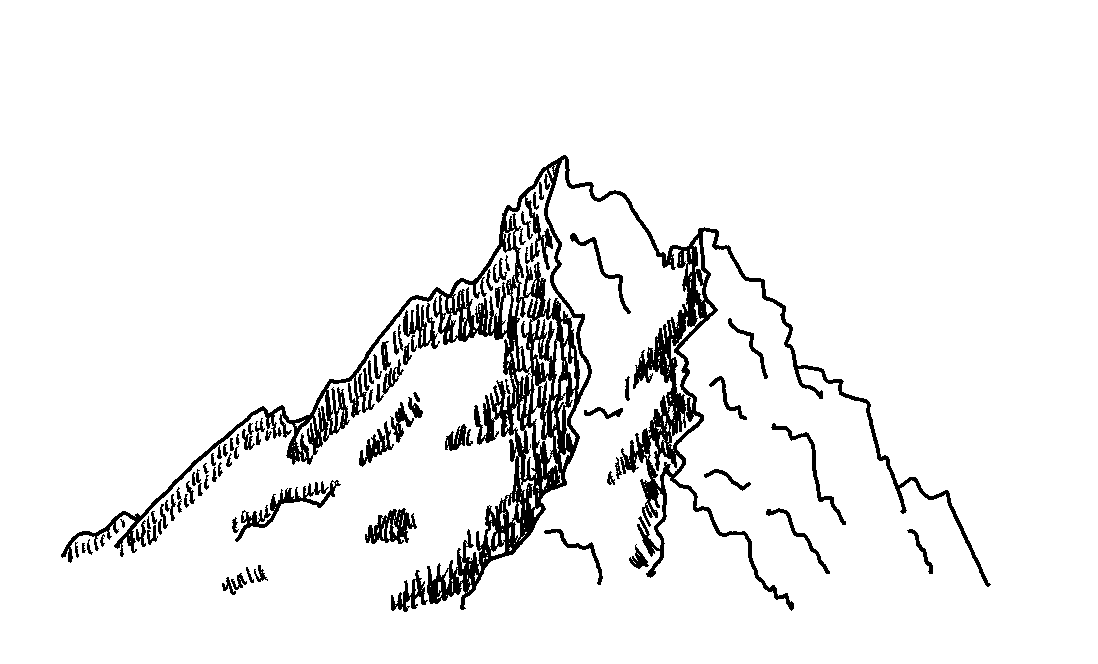
\includegraphics[width=0.4\textwidth]{images/mtn.png}
    \caption*{Gradient ascent.}
\end{figure}

These are course notes for the Winter 2024 rendition of CS M146: Machine Learning, taught by Professor Sriram Sankararaman. The credit for the template goes to Tyler Zhu. Almost none of what is written here is original.

\tableofcontents 

\newpage

%TODO: add in a cheat sheet of common formulas, distributions, etc. as we learn them. 
\section{Tuesday, January 9th}
One definition of machine learning could be: the study of algorithms that: \\
- improve their performance $P$, \\
- at some task $T$, \\
- with experience $E$. \\
Then a well defined learning task could be given by $(P, T, E)$ (Tom Mitchell, 1998). As an example, $T$ could be recognizing hand-written words, $P$ could be the percentage of words correctly classified, and $E$ could be a database of human-labeled images of hand written words (MNIST). Another definition could be: predicting the future based on the past (Hal Daume III). \\\\
Why are we interested in machine learning, and when do we use machine learning? There are many reasons, but a good set of them could be: \\
1) Lots of data (experience) \\
2) Trends and patterns from the data (prediction) \\
3) Measures of performance (benchmarks) \\
4) Humans lack expertise (navigating on mars) \\
5) Humans have expertise, but its unclear why or how it could be leveraged (i.e., vision, speech) \\
6) Efficiency compared to humans; algorithms must be customized (i.e., recommender systems, medical diagnosis) \\\\
Another valid reason to be interested in machine learning is how fundamental it is to modern-day deep learning and other fields. The goals of the course are to learn about both \\
- Fundamental concepts and algorithms \\
- Common techniques/tools used (theoretical understanding \textit{and} practical implementation/best practices \\\\
Applications of machine learning are broad. Some examples of technologies largely enabled, improved, or influenced by machine learning ideas include autonomous cars, computer vision, speech recognition, machine translation, natural language understanding, game playing, and medicine. 
\subsection{Types of Learning}
In machine learning, there are three main types of learning. \\
\textbf{Supervised (inductive) learning:} (``Learn with a teacher''). In supervised learning, we're \\
- Given \textit{labeled} training instances (or examples), with the \\
- Goal to learn a function (mapping) that predicts the label for \textit{test} instances \\
\textbf{Unsupervised learning:} (``Learn \textit{without} a teacher''). In unsupervised learning, we're \\
- Given \textit{unlabeled} inputs, with the \\
- Goal of learning some instrinsic \textit{structure} in the inputs \\
\textbf{Reinforcement learning:} (``Learn by interacting''). In reinforcement learning, we're \\
- Given an \textit{agent} that interacts in an \textit{environment} (has a set of states), with the \\
- Goal of learning a \textit{policy} (function from state to action) that maximizes an agent's reward \\\\
A good example of supervised learning is \textbf{regression}. In regression problems, we're given instance-label pairs $(x_1, y_1), (x_2, y_2, \ldots, (x_n, y_n)$ with the goal of learning a function $f(x)$ to predict $y$ given $x$. When $y$ is \textit{real valued}, this is called \textit{regression}. An example of a regression problem is predicting a building's rent given its square footage. \\

Another example of supervised learning is \textbf{classificaton}. With a similar setup to regression, namely given instance-label pairs and the goal of learning a function $f(x)$ to predict $y$ given $x$, if $y$ is \textit{categorical}, this is called \textit{classification}. An example of a classification problem is predicting if a breast cancer image is malignant or benign. \\\\
Importantly, our $instances$ (single observations/data points) can have multiple features. Mathematically, this means that $x$ can be multi-dimensional. For example, in the problem of predicting rent in a city, a single house (instance) could have multiple features: number of bedrooms, number of bathrooms, square footage, etc. \\\\
In unsupervised learning, we are given instances $x_1, x_2, \ldots, x_n$ \textit{without} the corresponding labels (they may or may not exist!), and we are interested in finding a hidden structure behind $x$. One example of this is the clustering problem, i.e., in genomics, grouping individuals by genetic similarity. \\\\
In reinforcement learning, an agent interacts with an environment, given a sequence of states, corresponding actions, and receiving (delayed) rewards or penalties based on the actions. The goal is for the agent to learn a policy that maximizes the cumulative reward over time. One example is DeepMind's \textit{AlphaGo}, which relies heavily on reinforcement learning ideas to play superhuman-level Go. 
\subsection{The Learning Problem}
A highly important concept is understanding the \textit{framing} of a learning problem. The first step is the representation of instances/examples. The representation chosen is how machine learning algorithms ``view'' the data. Typically, instances have corresponding features, which can be thought of as the questions we can ask about the instances. The next step is the learning algorithm itself, which can be highly different based on the problem. In general, during learning, we want to learn a model of what distinguishes the instances (in supervised learning, what distinguishes between their labels, i.e., a condo vs. a mansion) based on the features. Then, when a model sees a specific instance it has not seen before, it should (hopefully) output a good prediction as to what type (label) of instance it is. \\\\
The goal of learning (and therefore learning algorithms) is to be able to \textit{generalize} from training data. However, this assumes that the training data and test data are related, and ideally represent the real-world problem it was trained to solve. Additionally, how we measure this performance depends on the problem we are trying to solve. Mathematically, this means choosing or defining a loss/cost function, $L(y, \hat{y})$ that tells us how ``bad'' the prediction of $y$ is compared to the true value ($\hat{y}$). In regression, we could choose to use squared loss:
$$
L(y, \hat{y}) = (y - \hat{y})^2
$$
and in classification, we could use a simple piecewise function
$$
L(y, \hat{y}) = 
\begin{cases} 
      0 & y = \hat{y} \\
      1 & \text{otherwise}
\end{cases}
$$
Futhermore, we can use the \textit{probabalistic model} of learning, where there is some unknown probability distribution $p$ over our instance-label pairs (called the data generating distribution), which can be thought of as the data which we could expect to see (``characterizes experience''). \newpage Specifically, we have a \textbf{problem setting}, which consists of \\
- A set of possible instances $X$, \\
- A set of possible labels $Y$, \\
- An unknown target function/mapping $f: X \rightarrow Y$, \\ 
- And a set of function hypotheses $H = \{h | h: X \rightarrow Y \}$, \\
an \textbf{input}, which are training instances drawn from the (unknown) data generating distribution $p$, and an \textbf{output}, which is $h \in H$ that best approximates $f$. The hope is that $h$ should do well (measured by our choice of loss) on future/unseen instances. Mathematically, $h$ should have low expected (test) loss, 
$$
\mathbb{E}_{(x, y) \sim p} [L(y, h(x))] = \sum_{x, y} p(x, y) L(y, h(x))
$$
Unfortunately, we don't know what $p$ is, but we are given samples drawn from $p$. So, we can instead utilize the idea of \textbf{empirical risk minimization} (ERM). Although we don't know the true distribution of the data, we can estimate/approximate the empirical risk (training error). In this utilization, though, we assume that both the training data and the test set are generated from the same distribution - which can make the training error zero by \textit{memorizing} our data examples, and making its performance on unseen data (typically) very poor. Mathematially, we can define the empirical risk/training error as
$$
\frac{1}{n} \sum_{i = 1}^n L(y_i, h(x_i))
$$
As an example, in regression, we have an \textit{infinite} choice of hypotheses (the degree of the polynomial we will use to fit the data). To deal with this, we choose a loss function (i.e., squared loss, found above) and measure the performance of different degree-$n$ polynomials on unseen test data. To summarize, the learning problem is that we have access to training error, but really care about the test error. Additionally, our learned functions needs to generalize beyond the training data.
\subsubsection{Key Issues in Machine Learning}
There are some important, key issues in machine learning. Namely, there are the issues of \\
\textbf{Representation} (how we choose a hypothesis space). Often, we use \textit{prior knowledge} to make this choice. \\
\textbf{Optimization} (how we find the best hypothesis in this space). This is primarily an \textit{algorithmic} question. \\
\textbf{Evaluation} (how we gauge performance of a hypothesis on unseen data). This question is the main topic of \textit{learning theory}. 
\subsection{Summary}
To summarize, we formalize a learning problem by choosing a loss function $L$ and learning a function (hypothesis) $h$ that has low expected loss on samples from an unknown data generating distribution $p$. In this way, learning can be viewed as \textit{approximating} a function or mapping, and this approximation process can be viewed as searching through the space of hypotheses (representations of functions) for one that best fits a set of training data. Different learning methods assume different hypothesis soaces or employ different ``search techniques.'' However, the fundamental difficulty is that we are interested in expected loss, in order for the chosen function to generalize. 
\newpage

\section{Thursday, January 11th}
\subsection{Decision Trees}
In many machine learning problems, we are interested in an interpretable ways to make predictions. One possible machine learning algorithm that can accomplish is the \textbf{decision tree}. We will primarily view decision trees as models that can be used for classification (multi-class or binary), but we can also do regression with decision trees. In a decision tree, we ``walk down'' the  decision tree starting from the root, taking a specific instance and checking its attributes to decide which nodes and edges to travel through, until we get to a leaf node (prediction). Specifically, the general setup is to have \\
- Each internal node is an attribute/feature that a data example has. \\
- Each edge is a ``value'' that belongs to an attribute that a data example can take on. \\
- Each leaf node is a prediction/label. \\
As an example, take the following tree: 
\begin{figure}[h!]
    \centering
    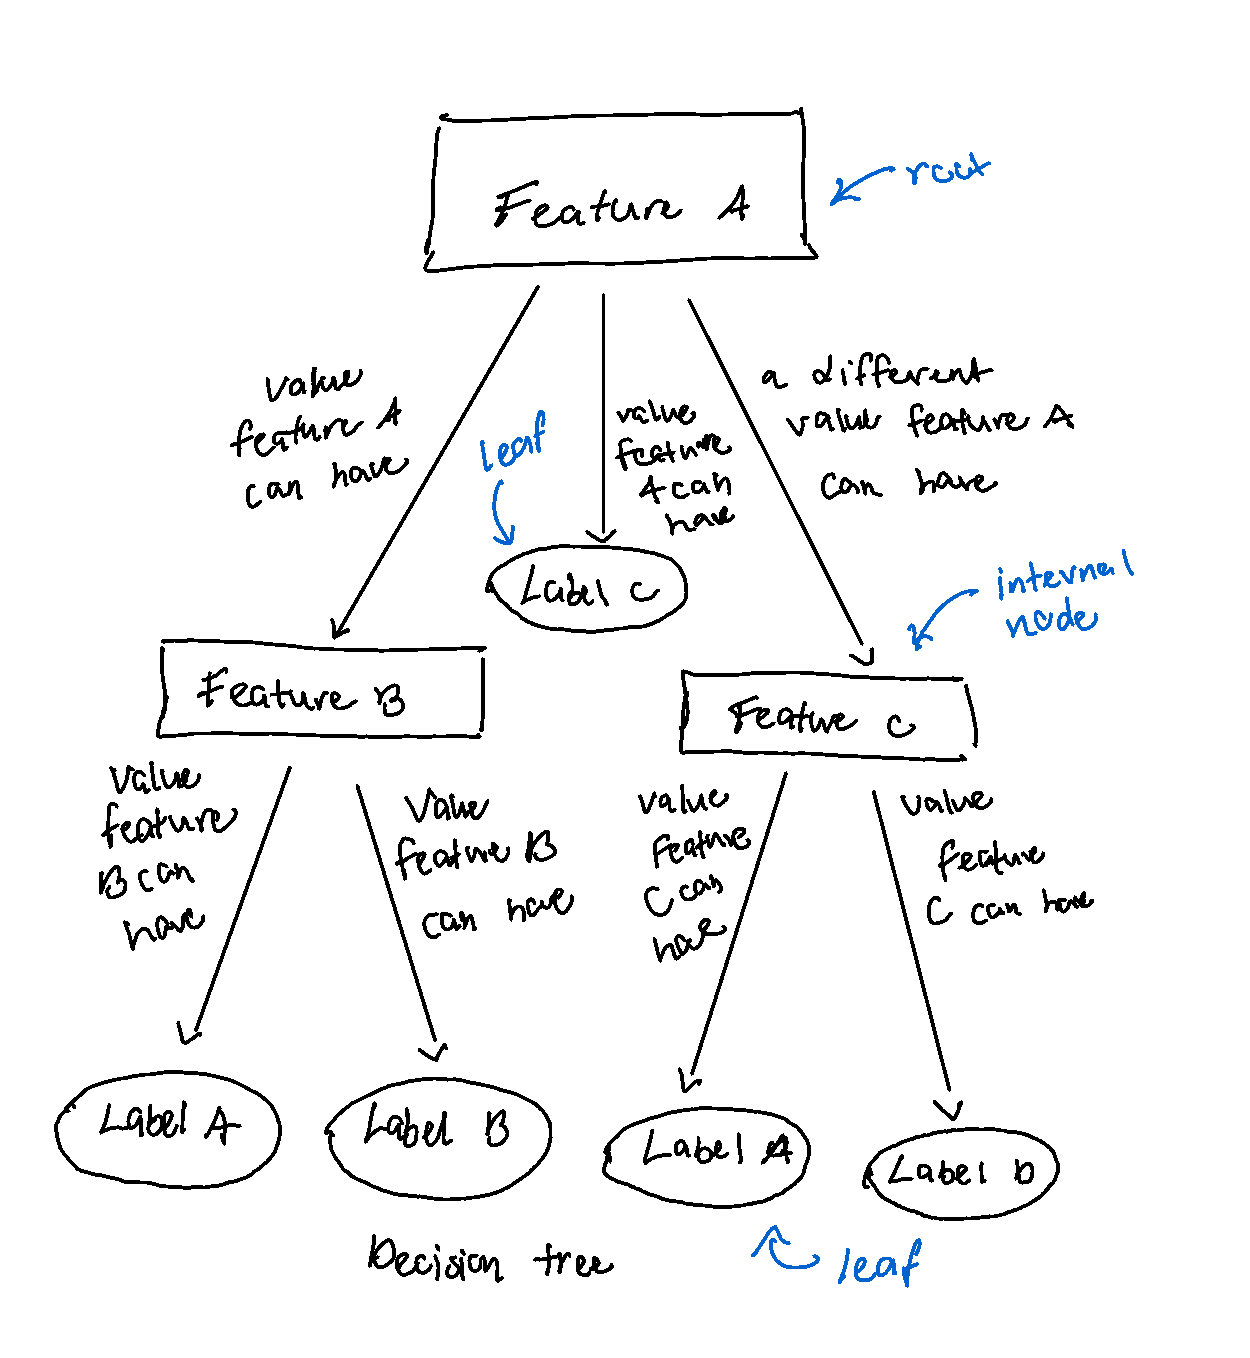
\includegraphics[width=0.7\textwidth]{images/decisiontree.png} % Adjust width as needed and provide the correct path to the image
    \caption{A generic decision tree.}
    \label{fig:q1_image}
\end{figure}
A decision tree can also be thought of as a model that partitions the feature space by recursively splitting it into subsets based on the values of features (edges). Then, the space that edges define or ``enclose'' constitute a prediction (leaf node). Then, we have the following setup: \\
- A set of possible instances $X$; each instance $x \in X$ is a feature vector \\
- A set of possible labels $Y$; $Y$ is discrete valued \\
- An unkown target function $f : X \rightarrow Y$ \\
- A set of hypotheses $H = \{ h | h: X \rightarrow Y\}$; each hypothesis $h$ is a decision tree \\
- Goal: Train/induce/learn a function $h$ that maps instance to label
\newpage Generally, there are three things to learn: \\
1. The structure of the tree (if we remove the ``text'', what does the tree look like?; what about our nodes?) \\
2. The values at the edges (choice of splitting, better learning) \\
3. The values for the leaves (predictions) \\\\
For any given dataset, there are many possible decision tree. We could build a very large tree, but it would likely overfit (discussed later). So, we take on an inductive bias (``hypothesis'', in a way) by Ockham's razor: the simplest consistent explanation is best. Ideally, we want the smallest decision tree that correctly classifies all training examples, but this problem is NP-hard. Instead, we greedily construct a decision tree that is fairly small. \\\\
An important decision in learning a decision tree are choosing good features as nodes, in order to do well on metrics we choose (accuracy, lower error, generalizability, etc). The algorithm that we examine in class is the \textbf{ID3 Algorithm}, which selects the feature(s) with the largest information gain. The key idea behind the ID3 algorithm is that gaining information reduces uncertainity. In order to measure uncertainy, we introduce the idea of \textbf{entropy}. 
\subsubsection{Entropy}
\begin{definition}
    if a random variable $X$ has $k$ different values $a_1, a_2, \hdots, a_k$, its \emph{entropy} is given by
    \[H[X] = -\sum_{k = 1}^KP(X = a_k)\log_2 \left[P(X = a_k) \right] \]
Note that the base of the log does not necessarily have to be two, but if the base is two, the unit of entropy is known as the ''bit.'' The higher the \emph{entropy} (corresponding to the uncertainty of a random variable with a specific probability distribution), the less ``confident'' we are in its outcome. 
\end{definition}
Similarily, and more importantly to the \textbf{ID3 algorithm}, we have the concept of \textbf{conditional entropy}.
\subsubsection{Conditional Entropy}
\begin{definition}
Given two random variables $X$ and $Y$, their \emph{conditional entropy} is defined as 
\[H[Y|X] = \sum_k P(X = a_k)H[Y|X = a_k] \]
\end{definition}
Finally, combining the two, we have \textbf{information gain}, which is the expected reduction in entropy of the target variable $Y$ due to splitting on the feature $X$. This is also called \textbf{mutual information} between $Y$ and $X$.
\subsubsection{Information Gain} 
\begin{definition}
We define information gain as
\[\text{\textbf{GAIN}} = H[Y] - H[Y|X] \]
\end{definition}
\newpage
Consider the following two possible splits.
\begin{figure}[h!]
    \centering
    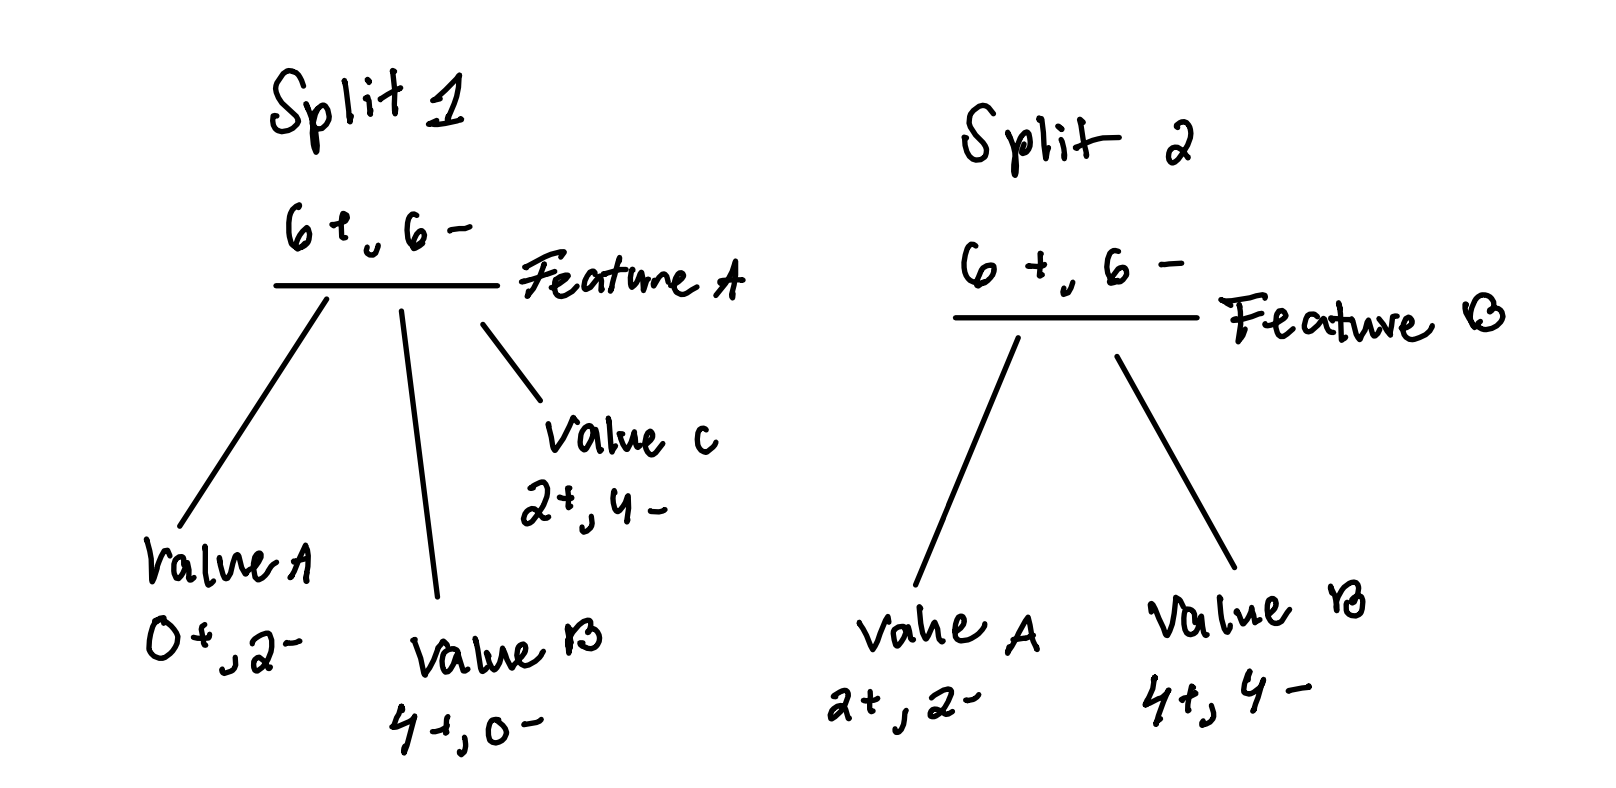
\includegraphics[width=0.7\textwidth]{images/infogain_ex.png} % Adjust width as needed and provide the correct path to the image
\end{figure}
\\We will calculate the conditional entropy and the information gain. Note that $+$ is for positive example, $-$ is for negative example. Starting with split 1, we have the entropy for the branch with value A to be
$$
H[\text{Value A branch}] = -\left(\frac{0}{0 + 2}\log_2\left(\frac{0}{0 + 2}\right) + \frac{2}{0 + 2}\log_2\left(\frac{2}{0 + 2} \right) \right) = 0
$$
The entropy for the branch with value B is
$$
H[\text{Value B branch}] = -\left(\frac{0}{0 + 4}\log_2\left(\frac{0}{0 + 4}\right) + \frac{4}{0 + 4}\log_2\left(\frac{4}{0 + 4} \right) \right) = 0
$$
finally the entropy for the branch with value C is
$$
H[\text{Value C branch}] = -\left(\frac{2}{4 + 2}\log_2\left(\frac{2}{4 + 2}\right) + \frac{4}{4 + 2}\log_2\left(\frac{4}{4 + 2} \right) \right) \approx 0.92
$$
Then the conditional entropy also includes the ``weightedness" of each branch, so we have
$$
H[\text{Target}|\text{Feature A}] = \frac{2}{12}(0) + \frac{4}{12}(0) + \frac{6}{12}(0.92) \approx 0.45
$$
and thus our information gain for splitting on feature A is
$$
\textbf{GAIN} = H[Y] - H[Y|X] = 1 - 0.45 = 0.55
$$
Now we turn to split 2. We have the entropy for the branch with value A to be
$$
H[\text{Value A branch}] = -\left(\frac{2}{2 + 2}\log_2\left(\frac{2}{2 + 2}\right) + \frac{2}{2 + 2}\log_2\left(\frac{2}{2 + 2}\right) \right) = 1
$$
and similarily for the branch with value B,
$$
H[\text{Value B branch}] = -\left(\frac{4}{4 + 4}\log_2\left(\frac{4}{4 + 4}\right) + \frac{4}{4 + 4}\log_2\left(\frac{4}{4 + 4}\right) \right) = 1
$$
then our conditional entropy is
$$
H[\text{Target}|\text{Feature B}] = \frac{4}{12}(1) + \frac{8}{12}(1) = 1
$$
and finally our information gain for splitting on feature B is
$$
\textbf{GAIN} = H[Y] - H[Y|X] = 1 - 1 = 0
$$
which is terrible (we gained no information), because the data after using split 2 is the same distribution as before.
\newpage
Now that we know how to train a decision tree, we are interested in its performance. Since decision tree learning / training is based on a greedy algorithm, decision trees can tend to \textbf{overfit}. For this reason, we have as our \textit{inductive bias} that we prefer shallow trees. However, we need to be careful with the tree depthy that we pick. If the depth is too high (``too deep''), we may overfit on the data (memorizing the training data, not learning). If the depth is too low (``too shallow''), we may underfit and not learn enough to have meaningful performance. Then, for this reason, max depth is a \textbf{hyperparameter} that we would need to tune.
\subsubsection{Hyperparameters}
\begin{definition}
A \emph{hyperparameter} is a configuration setting external to a machine learning model that cannot be learned from training data but is set prior to the training process. For our decision tree, the \emph{max depth hyperparameter} controls other parameters of the tree (number of nodes, levels, etc).
\end{definition}
In our decision tree, there are a couple possible reasons for overfitting:
\begin{enumerate}
  \item Noisy data
    \begin{enumerate}
      \item Two instances could have the same feature values but different class labels
      \item Some of the feature or label values could be incorrect (mislabeled)
    \end{enumerate}
  \item Some feature could be irrelevant to classification (unncecessary ``learning'')
  \item The target variable is non-deterministic in the features
    \begin{enumerate}
      \item In general, it is impossible to measure all the variable needed to perfectly predict (or even predict well at all!). Then, the target variable is not uniquely determined by the input feature values.
    \end{enumerate}
\end{enumerate}
In general, the training error when learning a decision tree is not guaranteed to be zero (even loss so if you want to avoid overfitting). However, our decision tree learning procedure \textit{always} increases training set accuracy, but this has no guarantee of decreasing test accuracy. The most straightforward to detect overfitting is to compute an accuracy score (or other metric) on test data that we store away (ideally, from the same distribution that models the real-life task or problem). The only downside to this is that we will have less training data. 
\subsubsection{MISSING SUPPLEMENTAL}
Should add material and graphics on overfitting (see slides), and other metrices (F1, sensitivity/specificity (precision/recall), bias/variance, ROC, AUC). 
\subsection{Cross-Validation}
Cross-validation is another independent dataset that we can predict on, which can serve the same purpose as the test set. However, the cross-validation set is more general, and is also used as dataset to tune hyperparameters, typically through a process known as \textbf{k-fold cross validation}.
\newpage
\subsubsection{K-Fold Cross-Validation}
\begin{definition}
In \emph{k-fold cross validation}, we
\begin{enumerate}
  \item Randomly partition the full data set of $N$ instances into $K$ disjoint subsets (roughly of size $\frac{N}{K}$).
  \item We choose each fold in turn as the test set, and train our model on the other folds, and subsequently evaluate our learned model on this cross-validation set.
  \item We finally compute average statistics over $K$ test performances. 
\end{enumerate}
When $K = N$, this is known as ``leave-one-out cross validation'' or LOOCV for short. When tuning hyperparameters, we would repeat k-fold cross validation (with our same choice of k) across the choice of hyperparameters we are interested in, and choose the hyperparameter such that \textit{on average}, the model performs the best. 
\end{definition}
In order to avoid overfitting, with a special focus on avoiding overfitting for decision trees, we can
\begin{enumerate}
  \item Get more training data
  \item Remove irrelevant features
  \item Force the decision tree to be simple via \textit{decision tree pruning}:
    \begin{enumerate}
      \item We can prune \textit{while} building the tree (early stopping) 
      \item Or we can prune \textit{after} building the tree (post pruning)
    \end{enumerate}
\end{enumerate}
If we prune while building the tree (early stopping), when classifying a new instances, we would label the leaves of the smaller trees (in order to make a decision) with the \textit{majority} of the training samples' labels.
\subsection{Advantages and Disadvantages of Decision Trees}
To summarize and finish the discussion on decision trees, we compare the advantages and disadavantages of decision trees below.
\subsubsection{Advantages} 
\begin{enumerate}
  \item Easily interpretable by humans (providing the tree is not too deep)
  \item Computationally efficient
    \begin{enumerate}
      \item For numerical we features, we could split on any feature, with any threshold
      \item Howeverm for a given feature, the only split points we need to consider are the $n$ values in the training data for this feature
      \item If we sort each feature by these $n$ values, we can quickly compute our metric of interest (information gain/conditional entropy). This takes $O(dn \log n)$ time, where $d$ is the number of continuous features and $n$ is the number of examples.
    \end{enumerate}
  \item Handles both numerical and categorical data
\end{enumerate}
\subsubsection{Disadvantages}
\begin{enumerate}
   \item Heuristic training techniques
     \begin{enumerate} 
       \item Finding a tree that minimizes empirical error is \emph{NP-hard} 
       \item We resort to greedy approaches (left alone, will overfit)
     \end{enumerate}
\end{enumerate}
With this, we end our discussion on decision trees!
\newpage
\section{Tuesday, January 16}
One very useful method to identify the right learning model to use is \textit{visualization}. Below is a visualization for the Iris dataset, which has four features and three classes. Each colored point is an instance, and different features are plotted against each other. 
\textbf{MISSING VISUALIZATION}
Notably, some of the data is already well seperated. Then, as an inductive bias, we can consider the label of the instance to be similar to the labels of nearby instances. This motivates the next learning algorithm, \textbf{nearest neighbors classification}.
\subsection{Nearest-Neighbors}
\subsubsection{Nearest Neighbor classification}
\begin{definition}
  In \emph{nearest neighbor classification}, we training by simply storing the entire training set. In prediction (testing), however, we have
$$
\textbf{x}(1) = \textbf{x}_{\text{nn}(\textbf{x})}
$$
where nn$(x) \in [N] = \{1, 2, \hdots, N \}$, i.e., the index to one of the instances. Namely,
$$
\text{nn}(\textbf{x}) = \text{argmin}_{n \in [N]} ||\textbf{x} - \textbf{x}_n||_2^2
$$
then our classification rule is
$$
y = h(\textbf{x}) = y_{\text{nn}(\textbf{x})}
$$
\end{definition}
However, the Euclidian norm $|| \cdot ||$ (or $L_2$ distance) is not the only notion of distance we can use, and our choice of distance can change the results of the nearest neighbors classification. Of note is the $L_1$ distance (aka Manhattan distance, city block distance), which is simply the absolute value, or notably in our case we would have
$$
\text{nn}(\textbf{x}) = \text{argmin}_{n \in [N]} \sum_{d = 1}^D |x_d - x_{nd}|
$$
So far, we have only discussed real-valued features. But if we are interested in binary features, we can simply choose $0$ and $1$ as our positive and negative classes, respectively. Furthermore, if we had categorical features with $V$ values, we would map to $V$-binary features. This is also known as \textbf{one-hot encoding}, where would create subsequent bit strings with all zeros except for a single 1. 
\\\\
Additionally, for every instance, we can determine its label using the NNC rule above. This gives rise to a \textbf{decision boundary} that partitions the space into different regions. Unlike decision trees, however, this decision boundary is likely more jagged to smoother (as we will see later) rather than enclosed.
\newpage
\subsubsection{K-Nearest Neighbors}
\begin{definition}
  In \emph{k-nearest nieghbors}, we simply increase the number of neighbors to use, and for each neighbor that we consider, we remove it when considering the next $n$th nearest neighbor. I.e., we have
\begin{center}
  \begin{enumerate}
    \item 1-nearest neighbor: $\text{nn}_1(\mathbf{x}) = \text{argmin}_{n \in [N]} ||\mathbf{x} - \mathbf{x}_n||_2^2$
    \item 2nd-nearest neighbor: $\text{nn}_2(\mathbf{x}) = \text{argmin}_{n \in [N] - \text{nn}_1(\mathbf{x})} ||\mathbf{x} - \mathbf{x}_n||_2^2$
    \item 3rd-nearest neighbor: $\text{nn}_3(\mathbf{x}) = \text{argmin}_{n \in [N] - \text{nn}_1(\mathbf{x}) - \text{nn}_2(\mathbf{x})} ||\mathbf{x} - \mathbf{x}_n||_2^2$   
  \end{enumerate}
\end{center}
Then the set of k-nearest neigbors is 
$$
\text{knn}(\textbf{x}) = \{\text{nn}_1(\textbf{x}), \text{nn}_2(\textbf{x}), \hdots , \text{nn}_k(\textbf{x})\}
$$
notably, if we let $\textbf{x}(k) = \textbf{x}_{\text{nn}_k(\textbf{x})}$, then
$$
||\vecx - \vecx(1)||_2^2 \leq ||\vecx - \vecx(2)||_2^2 \leq \hdots \leq ||\vecx - \vecx(k)||_2^2
$$
Finally, our classification rule for k-nearest neighbors is as follows:
\begin{center}
\begin{enumerate}
  \item Every neighbor votes: suppose $y_n$ (the label) for $\vecx_n$ is $c$, then a vote for $c$ is 1, and a vote for $c' \neq c$ is 0. We then use an \textit{indicator function} $\mathbb{I}(y_n == c)$ to represent the following.
  \item We first aggregate everyone's vote: 
    $$
    v_c = \sum_{n \in \text{knn}(\textbf{x})} \mathbb{I}(y_n == c) \ \ \forall \ \ c \in [C]
    $$
  \item Then we label with the majority:
    $$
    y = h(\vecx) = \text{argmax}_{c \in [C]}(v_c)
    $$
\end{enumerate}
\end{center}
\end{definition}
Note that as $k$ increases, the decision boundary becomes smoother and smoother. \textbf{MISSING VISUALIZATION}
Additionally, we can preprocess the data, namely normalizing the data to have zero mean and unit standard deviation in each dimension in order to improve performance. Specifically, we do the following:
\begin{enumerate}
  \item Compute the mean for each feature
    $$
    \bar{x}_d = \frac{1}{N} \sum_n x_{nd}
    $$
  \item Compute the standard deviations in each feature
    $$
    s_d^2 = \frac{1}{N - 1} \sum_n (x_{nd} - \bar{x}_d)^2
    $$
  \item Use the two statistics to scale the feature accordingly:
    $$
    x_{nd} \leftarrow \frac{x_{nd} - \bar{x}_d}{s_d}
    $$
\end{enumerate}
There are many ways to normalize data, and we would need to try different choices and pick them using cross-validation.
\subsection{Advantages and Disadvantages of K-Nearest Neighbors}
\subsubsection{Advantages}
\begin{enumerate}
  \item Computationally, simple and easy to implement: just store the dataset and compute the distances.
\end{enumerate}
\subsubsection{Disadvantages}
\begin{enumerate}
  \item Computationally intensive for large scale problems: $O(ND)$, where $N$ is the number of data points/instances, and $D$ is the number of features, in order to label a single instance.
  \item We need to ``carry'' the training data around; without it, we cannot classification. This is known as a \textit{nonparametric} method.
  \item Choosing the right distance measure and $k$ can affect performance; requires hyperparameter tuning.
\end{enumerate}

\end{document}

%%% Local Variables:
%%% mode: latex
%%% TeX-master: t
%%% End:

%%% Local Variables:
%%% mode: latex
%%% TeX-master: t
%%% End:
